\documentclass[times]{ettauth}
%\documentclass[times,doublespace]{ettauth}%For paper submission

\usepackage{acronym}
\usepackage{flafter}
\usepackage{listings}
\usepackage{xcolor}
\usepackage{multirow}
\usepackage{url}

\colorlet{punct}{red!60!black}
\definecolor{background}{HTML}{EEEEEE}
\definecolor{delim}{RGB}{20,105,176}
\colorlet{numb}{magenta!60!black}

\lstdefinelanguage{json}{
    basicstyle=\normalfont\ttfamily,
    numbers=left,
    numberstyle=\scriptsize,
    stepnumber=1,
    numbersep=8pt,
    showstringspaces=false,
    breaklines=true,
    frame=lines,
    backgroundcolor=\color{background},
    literate=
     *{0}{{{\color{numb}0}}}{1}
      {1}{{{\color{numb}1}}}{1}
      {2}{{{\color{numb}2}}}{1}
      {3}{{{\color{numb}3}}}{1}
      {4}{{{\color{numb}4}}}{1}
      {5}{{{\color{numb}5}}}{1}
      {6}{{{\color{numb}6}}}{1}
      {7}{{{\color{numb}7}}}{1}
      {8}{{{\color{numb}8}}}{1}
      {9}{{{\color{numb}9}}}{1}
      {:}{{{\color{punct}{:}}}}{1}
      {,}{{{\color{punct}{,}}}}{1}
      {\{}{{{\color{delim}{\{}}}}{1}
      {\}}{{{\color{delim}{\}}}}}{1}
      {[}{{{\color{delim}{[}}}}{1}
      {]}{{{\color{delim}{]}}}}{1},
}

\newcommand{\specialcell}[2][c]{%
  \begin{tabular}[#1]{@{}c@{}}#2\end{tabular}}

\begin{document}
\newacro{gdp}[GDP]{Gross Domestic Product}
\newacro{citysdk}[CitySDK]{Smart City Service Development Kit and its application Pilots}
\newacro{W3C}[W3C]{World Wide Web Consortium}
\newacro{POI}[POI]{Point of Interest}
\newacro{XML}[XML]{Extensible Markup Language}
\newacro{JSON}[JSON]{JavaScript Object Notation}
\newacro{REST}[REST]{Representational State Transfer}
\newacro{HATEOAS}[HATEOAS]{Hypermedia as the Engine of Application State}
\newacro{poi}[POI]{Point of Interest}
\newacro{gis}[GIS]{Geographical Information System}
\newacro{wg}[WG]{Working Group}
\newacro{iptc}[IPTC]{International Press Telecommunications Council}
\newacro{POIs}[POIs]{Points of Interest}



\runningheads{P. Cruz \emph{et al}}{CitySDK Tourism API - Building value around open data}

\articletype{Research Article - CONFIRM}

\title{CitySDK Tourism API - Building value around open data}
\author{Pedro Cruz\affil{1},
Ricardo Lopes Pereira\affil{2}\textsuperscript{,}\affil{1}\corrauth\,
Andr\'e Oliveira\affil{3} and 
Geert Monsieur\affil{4}}
\address{
 \affilnum{1}Instituto Superior T\'ecnico, Avenida Rovisco Pais 1, 1049-001 Lisboa, Portugal\\
 \affilnum{2}INESC-ID, Av. Prof. Dr. Cavaco Silva, 2744-016 Porto Salvo, Portugal\\
 \affilnum{3}ISA\\
 \affilnum{4}European Research Institute in Service Science (ERISS), Tilburg University, Warandelaan 2, 5037AB Tilburg, The Netherlands
}
\corraddr{E-mail: ricardo.pereira@inesc-id.pt}

\begin{abstract}
To be written later.
\end{abstract}

\maketitle

\acresetall
\section{Introduction}

\subsection{Motivation}
\label{s:motivation}
Tourism is a very important social, cultural and economic activity.
According to the World Tourism Organization, in 2012 tourism was responsible for 9\% of the world's \ac{gdp} and for 1 in every 11 jobs.
Tourism generated over 1.3 trillion US\$ in exports and 6\% of the world trade.
2012 was the year were the number of international tourists crossed the 1 billion mark\footnote{\url{http://media.unwto.org/sites/all/files/images/unwto1billioninfographic2.jpg} accessed June 17$^th$, 2013}.
More than half of international tourists elect Europe as their destination~\cite{unwto}.

As vacation time is limited and tourism is a costly activity, tourists wish to make the most of their stay.
There is an industry around travel guides, maps and advice.
This business is also being explored on the Internet and now is making the crossing to the ubiquitous smartphone.
The lower cost of entry when compared to traditional publishing should foster innovation, harvesting the opportunities brought forward by interactivity, positioning systems, wireless Internet access, augmented reality, social networks and crowd-sourcing. 
However, often the foundation for tourism applications is still quality, accurate, reliable information from authoritative sources.

National, regional and city authorities compile large amounts of information for use in their internal processes.
Municipalities understand the value of these data and many have gone through a multi-step process for sharing these data with tourists in order to improve their experience and attract them to the city.
First municipalities created applications (web or mobile) for sharing data with the tourists.
This approach is costly and unsuitable for most cities: the number of visitors is not large enough to recuperate the investment; municipalities are not software houses being unable to keep up with the pace of innovation. 
Furthermore, municipalities are limited in the types of applications they can provide: e.g. publishing negative opinions written by users about an attraction could expose them to liability.

Making data available to third parties is often a better investment and many entities have followed the open-data path.
With access to data, programmers bear the costs and risk, but are free to integrate data from several sources to create novel applications.
Market forces should drive innovation, creating the applications tourists want.
By publishing data, municipalities may also aid in the creation of local businesses exploiting this data.
Municipalities may still be forced to publish some applications on their own, should they deem them necessary but the market not. 
Still, the open-data model is not without flaws as each entity publishes different datasets using different data formats.
Applications will be restricted to the cities which provide the data required for that application.
Furthermore, programmers are forced to invest into dealing with the particularities of each data representation format, thus limiting the number of data sources which can be included into an application.
These factors will limit the cities covered by applications and thus their potential market, limiting the number and size of the investments.
The local nature of the applications will make them difficult for tourist to find, as they must find the particular applications for each city visited.
This problem is also felt for applications created by the municipalities.

The path taken by municipalities has also been traced by other entities related to tourism, such as national and regional governments, museums, concert halls or cultural events organisers.

\subsection{CitySDK}
\label{s:citysdk}

One of the most important goals in an European ICT PSP project entitled CitySDK, is to create an ecosystem in which the work of an application developer is facilitated by having unified and open city interfaces available across different cities in Europe. This means that it should be relatively easy for developers to make use of touristic data coming from multiple European cities, because in such an ecosystem data access is open and unified. CitySDK designs and develops three separate APIs: one for participation services (e.g. FixMyStreet), one for mobility data (e.g. public transport data) and one for  touristic information. In this article, we present the third API, referred to as the \emph{CitySDK Tourism API}, and show how it addresses the problems that municipalities and developers face (as described in Section \ref{s:motivation}). 

political awarenes
talk about the project
Common API when intersection among available data is small.
Flexibility to accommodate further usages not yet envisioned.

make way for delegation and common developer keys?




Talk about the project.

Briefly introduce the API.

\subsection{Document structure}
\label{s:structure}
This document is organised ...

This is an acronym expansion: \ac{citysdk}.



\section{Related work}
%add more description as we add more subsections
In this section we will present some of the studies and working groups related with smart cities in general.  

\subsection{\acf{W3C} \acf{POI} Working Group}
\label{section:poi-wg}
The \ac{W3C} is an international community where Member organizations, a full-time staff, and the public work together to develop Web standards. This community is led by Web inventor Tim Berners-Lee and CEO Jeffrey Jaffe. 

One of the its working groups is the \ac{W3C} POI~\cite{w3c-poi} and its mission is to develop technical specifications for the representation of \ac{POI} information on the Web. Its Core defines a generic, flexible, lightweight and extensible \ac{POI} data model, and one normative syntax for the data model based on \acf{XML}. Although \ac{XML} is the primary model for this specification, other formats are also possible, such as \acf{JSON}.

The data model is shown in Figure~\ref{fig:data-model}. A brief explanation is given next.

\begin{figure*}[!ht]
\centering
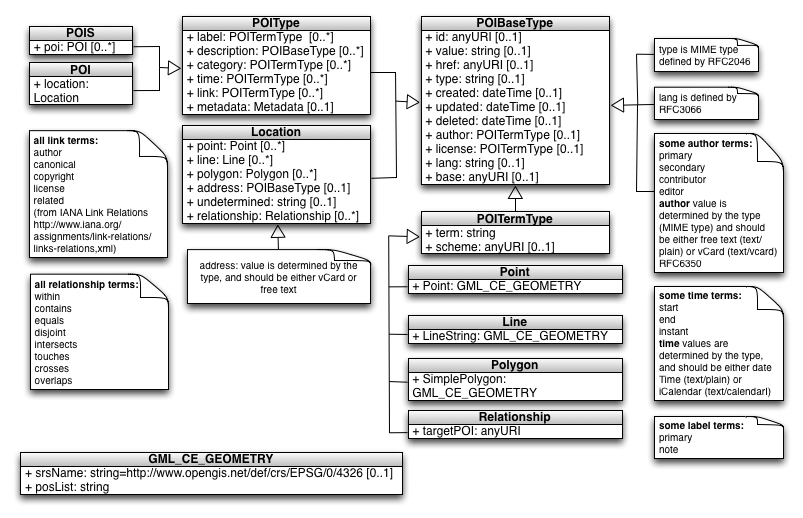
\includegraphics[width=0.9\textwidth]{images/uml}
\caption{W3C POI Core Data Model}
\label{fig:data-model}
\end{figure*}

The data model comprises of six entities:
\begin{itemize}
\item \textbf{POIBaseType} is the common entity from which the majority of POI entities are derived. It provides basic properties related with its authorship, licensing, modification dates and identification allowing each element to carry distinct information;
\item \textbf{POITermType} is an abstract entity derived from POIBaseType and adds properties for the management of categorical descriptions (such as the ones seen in category), link, label, author, license and time properties of POIType;
\item \textbf{POIType} is an abstract entity derived from POIBaseType and adds entities for describing, labeling, categorizing and indicating the time span of a POI or group of POIs. This entity also incudes linking elements to other POIs, external web resources or metadata;
\item \textbf{Location} is an entity the inherits from POIBaseType and provides a flexible description of the location of a POI. A Location can be represented using geodetic coordinates for the center of the POI, line, polygon, civic address,  undetermined (representing unresolved locations) or bounding box (relationship element);
\item \textbf{POI} inherits from POIType and adds the Location entity for describing the location of the POI;
\item Finally, \textbf{POIS} also derives from POIType and can have one or more children entities of type POI.
\end{itemize}

This model is used within our API to model various types of data, as described in section~\ref{section:w3cpoi}.

opendata

tourism and POI APIs

REST APIs?


\section{API Design}

In this section, we will describe some of the key features of the CitySDK Tourism API. We will describe the message format model, how the API is designed and some features that came along with it.

In order to address the challenges presented in Section \ref{s:challenges} and the broader goals of CitySDK (see Section \ref{s:citysdk}) a sound methodology is of critical importance to avoid the pitfalls of deploying an uncontrolled maze of APIs \cite{papazoglou2007,monsieur2012}. The well-adopted service oriented architecture (SOA) development lifecycle (SDLC) \cite{papazoglou2007} provides a solid foundation for service enablement in an orderly fashion so that services can be efficiently used in SOA-based smart city applications. The methodology is based on continuous refinement using a closed loop approach that facilitates designing SOA solutions (e.g. European smart city app) as assemblies of services in which each service assembly is a managed first class aspect of the solution, and, hence, amenable to analysis and change. Developers can then view an smart city app(lication) as a choreographed set of service interactions.

SDLC relies on three fundamental SOA design principles: coupling, cohesion and granularity. These design principles need to guarantee that services are self-contained and come equipped with clearly defined boundaries and interfaces to allow for service composability. Standards and reference models (e.g. W3C POI) are crucial in coping with such design principles. Typically, these standards improve SOA design by defining (sector-specific) business concepts that have an high-degree of cohesion and low-degree of coupling. The design of the tourism API is fundamentally based on W3C POI (see Section \ref{section:w3cpoi}). By reusing existing standards such as W3C POI the chance for adoption is substantially increased. Furthermore, it reduces coupling because developers are not bound to use message formats linked to a specific service implementation \cite{papazoglou2007}.

Before diving into a deeper description of the CitySDK API there are three fundamental aspects that should be mentioned. The API provides the following: four types of data models, methods to retrieve information concerning these same data models and also, methods and description fields that retrieve the relationships between each of them. Regarding the data models we provide the following:
\begin{itemize}
\item \textbf{\ac{POI}} describes various places in a given city, ranging from monuments and museums to eating places and cultural venues; 
\item \textbf{Event} describes cultural events that happened or are about to happen in the city;
\item \textbf{Itineraries} describe a group of \acp{POI} organized in such a way that they form an itinerary of a given topic, e.g., the life of a given person, the history of a given region or even just specific sightseeing spots;
\item \textbf{Categories/Tags} describe a list of available categories and tagging terms for each of the aforementioned models.
\end{itemize}

Each model can also be grouped into a list of its own type, that is, each data model has a listing model where each element is either a \ac{POI}, Event, Itinerary or a Category/Tag.

We now present the key features of the API.

\subsection{W3C POI Model in the API}
\label{section:w3cpoi}
As mentioned before, our API provides four data models: Points of Interest, Events, Itineraries and Categorization data. These models are mapped using the W3C POI Model presented in section~\ref{section:poi-wg}. We will now present how we modelled each data type.

The \textbf{\acf{POI}} are the most easily modelled element of the API. Since the W3C POI Model is specific for this type of data we used its already specified properties to map our data model. So, the Points of Interest are mapped and described by using the \textit{POI} entities directly. It should be mentioned that, since the \ac{POI} is somewhat very detailed and verbose, we defined two granularities for this element: a minimal description, that only includes the key essential properties and a complete model, which is the original W3C POI Data Model. The minimal model is used to map each element of a list of \ac{POI}. Such list is described by the \textit{POIS} entity, but it does not use the descriptive properties of \textit{POIType}.

The \textbf{Events} are modelled the same way the \acp{POI} were, but instead of having a \textit{Location} entity completly specified, we used the \textit{relationship} property of the same entity to relate a given Event to a \ac{POI} and ommited the \textit{address} and \textit{undetermined} properties. So, we have an Event completly described using the \textit{POI} entity and use the \textit{relationship} property to also specify and descibe the location of the Event. An Events list is modeled using the \textit{POIS} entity, much like the \acp{POI}, but it does not have a different granularity and the root name is \textit{event} instead of \textit{poi}.

The \textbf{Itineraries} is somewhat more complex. It is defined by using the \textit{POIS} entity and all of its descriptive properties. So, we have the description of the Itinerary itself by using the \textit{POIType} descriptive properties and have the group of \acp{POI} by using the \textit{poi} property named as \textit{pois} (so not to confuse with the mentioned list of \ac{POI}). It should be mentioned that these \acp{POI} are not the original \acp{POI}, but are described in the context of the Itinerary, though they include the relationship with its original counterpart, so to fetch the actual description. Finally and like the previous two, the Itineraries has a list associated with it. Much like the \ac{POI}, it has a second granularity - a minimal version - in which only the description of each Itinerary is included and their \acp{POI} are ommited.

The \textbf{Categories/Tags} are equal in nature, but a Category provides a recursive format that the Tags do not. Both borrow from the W3C POI Data Model, but their format is more specific to the needs of the API, rather than following the mentioned model. So, a Category simply follows the \textit{POIType} entity and allows recursiveness and a Tag borrows its properties from the \textit{POIBaseType} to specify a language and value.

At last, most of the terms used in the POITermType are the suggestions made by the working group itself. However, we've added three more terms regarding price, waiting time, occupation and accessibility information for handicapped people. Such terms are identified as X-citysdk/price, X-citysdk/waiting-time, X-citysdk/occupation and X-citysdk/accessibility-textual and X-citysdk/accessibility-properties, respectively.

The presented models are used in the message format of the API, in the format of \ac{JSON} (like we have seen previously).

\subsection{API Description}
\label{api-description}
The API follows the \ac{REST} architectural design~\cite{Fielding:2002:PDM:514183.514185}. Thus, we designed a RESTful API over HTTP using JSON. Hence, for each of the presented models we designed various methods to obtain certain data following certain parameters. Many of the parameters are common between the \acp{POI}, Events and Itineraries, such as the ability to search for each one of them using a categorical reference, a description or using coordinates. Also, we have provided limitation parameters to allow applications to lazy load the data presented by the API. Of course, there are some parameters that are specific to the data model, e.g., if we search using a description of the \acp{POI}, one can ask for either the minimal or complete version or in the case of the Events, we can search using time spans. Furthermore, and for both \acp{POI} and Events, one can also search for the relation of a single \ac{POI}/Event with other \acp{POI}/Events. One final method is the ability to search using QR Code or Barcodes. Using a single method and providing the textual or bar code information, we retrieve any POIs, Events or Itinerary that match such information.

As for the categorization models, we have provided methods to retrieve the categorical information for each of the aforementioned models by using a list parameter indicating which type of data we wish to retrieve. Such results can also be limited by using the same limitation parameters mentioned above.

Another feature of the API, and somewhat ignored by many REST systems, is complying to the \acf{HATEOAS} constraint of Fielding's dissertation. This constraint states that a client interacts with a network application entirely through hypermedia provided dynamically by the application servers. Therefore, it needs no prior knowledge about how to interact with any particular application or server beyond a generic understanding of hypermedia. We made use of this constraint in three ways:
\begin{enumerate}
\item From the entry URL - the only URL that the client needs to know - we present the resources made available by the visited server;
\item Each of the Data Models has an identification (specified by a base URL and ID) that allows to fetch information about that specific model;
\item The POIs, Events and Itineraries can be further described by using a \textit{described-by} (in the links property) which indicates an entry point to another server, which can provide further data on that specific entity.
\end{enumerate}

The mentioned resources indicate to the client, which models and which parameters are available in a given server. These models can be presented by the key-values found in the response message, e.g., if a \textit{find-poi} key is found, then the server supports \acp{POI}. As for the allowed searching parameters we have used the URI Template RFC~\cite{uri-template}. This way, we allowed a simple yet descriptive manner to indicate which parameters and which data is available and can be fetched.

This feature allowed our system to delegate responsibilities, as we will see in Section~\ref{delegation}.

\subsection{Delegation}
\label{delegation}

different roles: programmer, city, museum, world wide directory.


As mentioned in Section~\ref{api-description} we designed an API based on hypermedia content. Such feature allows the use of delegation between the various entities involved in the system: a world-wide directory containing the endpoints of CitySDK-enabled servers; the city servers providing CitySDK data; and a more granular server provided by museums or any other venues which give more detailed information about that specific \ac{POI}, Event or Itinerary. Figure~\ref{fig:delegation} shows a diagram of the interactions between each entity.

\begin{figure}[!ht]
\centering
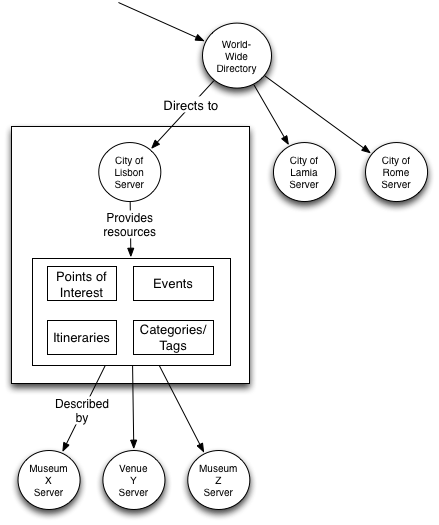
\includegraphics[width=0.4\textwidth]{images/delegation}
\caption{Delegation Model}
\label{fig:delegation}
\end{figure}

Further explaining the diagram, a client visits the world-wide directory and provides a given geodetic coordinates and an API key. The world-wide directory then directs the client based on the provided set of  coordinates and on the validation of the API key.

The client then visits the provided server address, in which the resources are provided, ending by querying the given server for any of the available data. 

At last, the client may further detail the information given by the server by visiting a museum or venue's server. Such server can be known if the provided resource has a \textit{described-by} parameter in the \textit{links} property containing the endpoint URL.

\section{Implementation}
Talk about Lisbon's implementation



\section{Evaluation}

\subsection{Proof of Concept Applications}
To further test our client libraries and API, we developed a group of key applications in various programming languages and frameworks.
The first application made use of the Java library. We developed an Android application which displays \acp{POI}, Events and Itineraries following a user's criteria, e.g using categorical information and/or using coordinates. It displays the retrieved data in both list and map format (in the case of the Itineraries, it would draw the route itself). Its main goal is to use the API to its fullest and demonstrate the various possibilities for applications.

We've also developed a set of applications making use of the JavaScript/jQuery library. These set of applications are an Event's calendar, and thus it makes specific use of Events and time/categories-related searches and a Map displaying all types of data models.

At last, we developed a Augmented Reality application using the Layar framework by developing a PHP web-server. Thus, in this case we used the PHP library. This application simply makes use of the position, camera and sensors of the user's device to display information about the surroundings and/or the building being displayed in the screen.

The Objective-C library was not ignored, since an application is being developed at the moment.

Evaluate the architecture from other perspectives: performance - http load balancing + delegation to multiple servers; ??



\section{Conclusions}


\acks
thank you

\bibliographystyle{wileyj}
\bibliography{references}

\end{document}


% Local IspellDict: "british"
% Local IspellPersDict: "~~/.ispell-English"

% Local Variables:
% mode: flyspell
% End:
